\subsection{Estudio y diseño de la aplicación de análisis de datos}
\label{sec:diseno-estudio}

El diseño de la aplicación de análisis de datos se ha realizado siguiendo una metodología centrada en el usuario. Para ello, 
se llevó a cabo un análisis de las necesidades de los usuarios, se definieron los requisitos de la aplicación y se diseñó la 
interfaz de usuario.

Entre las principales necesidades y requisitos de la aplicación destaca la importancia de que la visualización de los datos sea 
clara y sencilla, evitando la necesidad de conocimientos avanzados en análisis de datos para su uso.

El diseño de la interfaz de usuario sigue un enfoque sencillo y minimalista, con colores suaves y tipografía clara y legible. 
Se ha diseñado para ser intuitiva y fácil de usar, permitiendo al usuario acceder rápidamente a todas las funcionalidades. 
El foco está en la visualización de gráficos y datos, presentando la información de forma ordenada y consistente para facilitar 
su comprensión. Todas las gráficas y tablas comparten un estilo uniforme y limpio, evitando elementos visualmente recargados.

De forma similar a la OTT, este diseño sigue un enfoque modular, dividiendo la aplicación en componentes independientes que se 
comunican entre sí. Esto facilita el mantenimiento y la extensibilidad de la aplicación, ya que cada componente puede ser modificado 
o reemplazado sin afectar al resto. Además, el diseño modular permite la reutilización de código y la integración de nuevas funcionalidades.

\subsubsection{Estudio de las agrupaciones de datos}
\label{sec:diseno-agrupaciones}
Una vez definidos los requisitos de la aplicación y el diseño general, era importante estudiar qué agrupaciones de datos se podían 
lograr con las funcionalidades que ofrece Matomo y qué opciones de visualización se podían implementar.

Lo primero fue identificar qué tipos de gráficos eran necesarios soportar y diseñar. Tras analizar la entrega de datos que realiza 
Matomo, se decidió comenzar con el soporte para gráficos lineales, de barras, circulares y tablas. De esta manera, en función de la 
utilidad, periodo y enfoque de los datos, se podrán seleccionar diferentes tipos de gráficos para visualizar la información.

\paragraph{Páginas y secciones}
Posteriormente, se estudió qué páginas o apartados de la aplicación de análisis de datos podían implementarse. La primera página en la 
que se pensó fue el dashboard o página de inicio, donde se mostrarán gráficos que presenten información más general y resumida de los datos.


\begin{figure}[H]
    \centering
    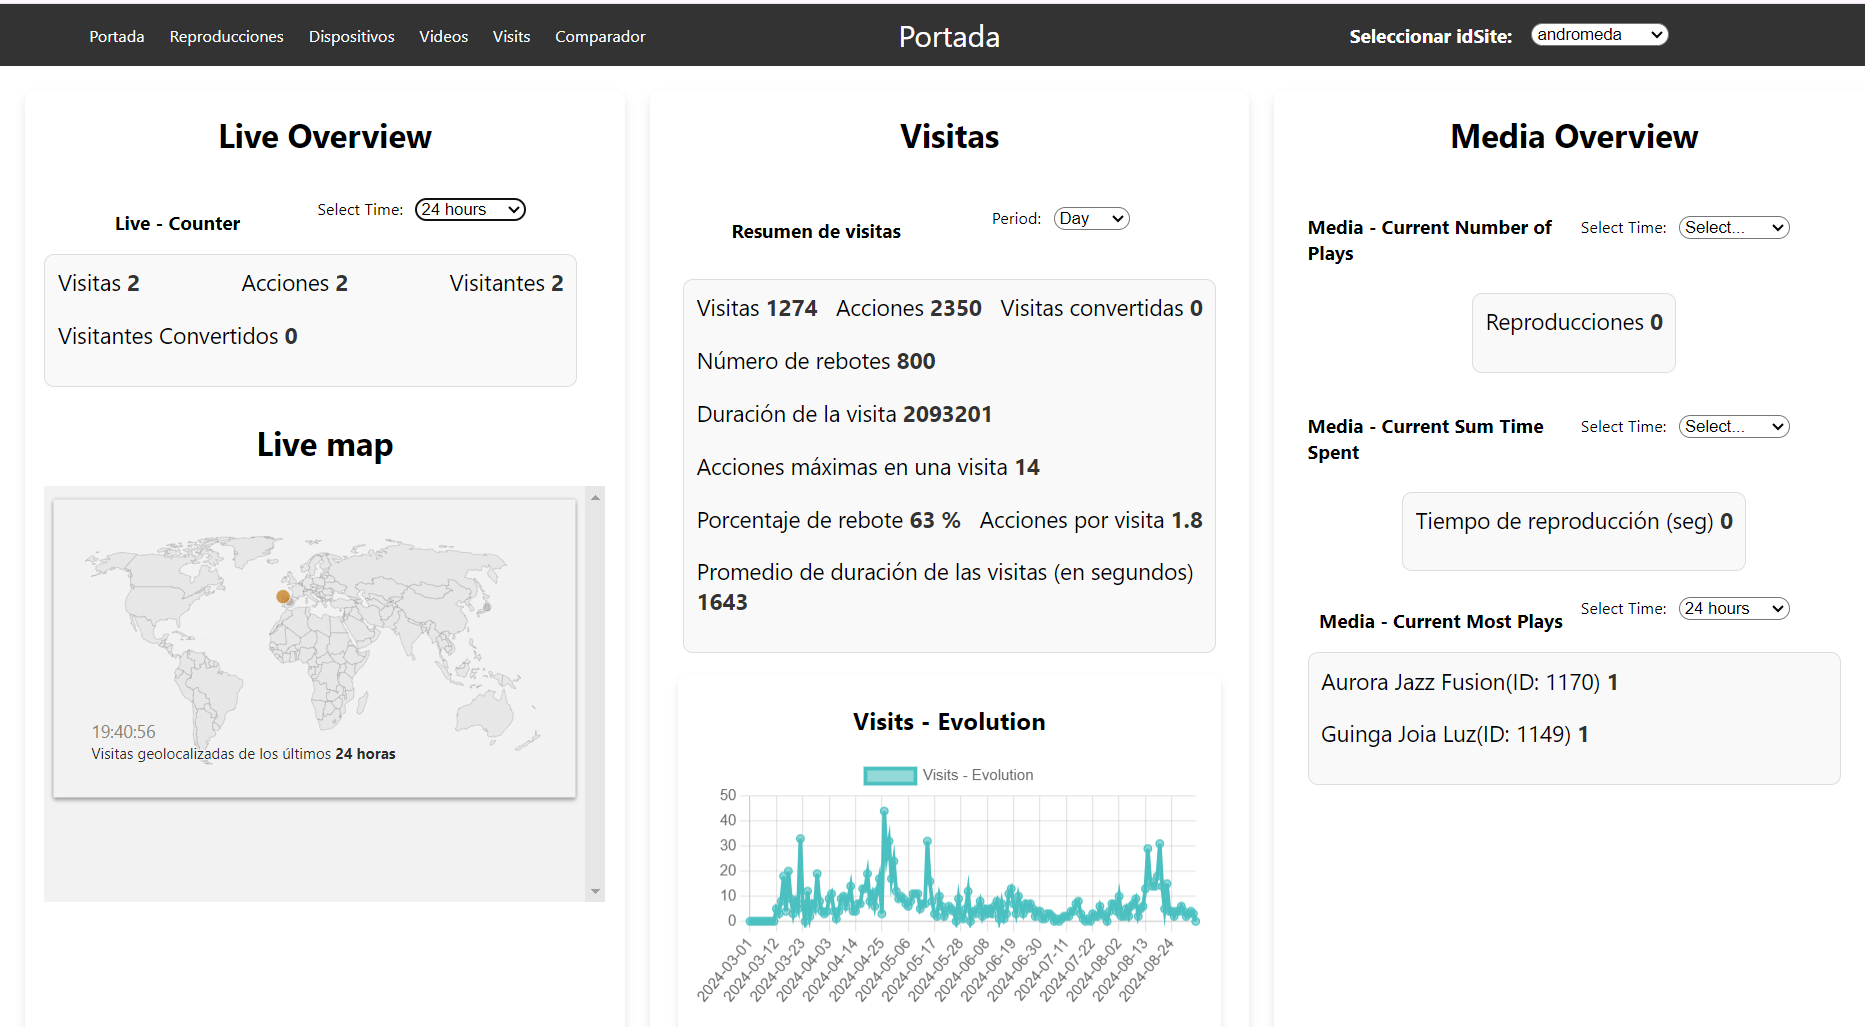
\includegraphics[width=0.8  \textwidth]{imaxes/dashboard.png}
    \caption{Página de inicio de la aplicación de análisis de datos}
    \label{fig:dashboard}
\end{figure}

Otra página considerada durante el análisis fue una que permitiera al usuario comparar gráficas de diferentes módulos. La idea 
era ofrecer al cliente la posibilidad de visualizar varias gráficas en una misma página, facilitando así el análisis de información 
en busca de patrones, tendencias o correlaciones entre los datos.

\begin{figure}[H]
    \centering
    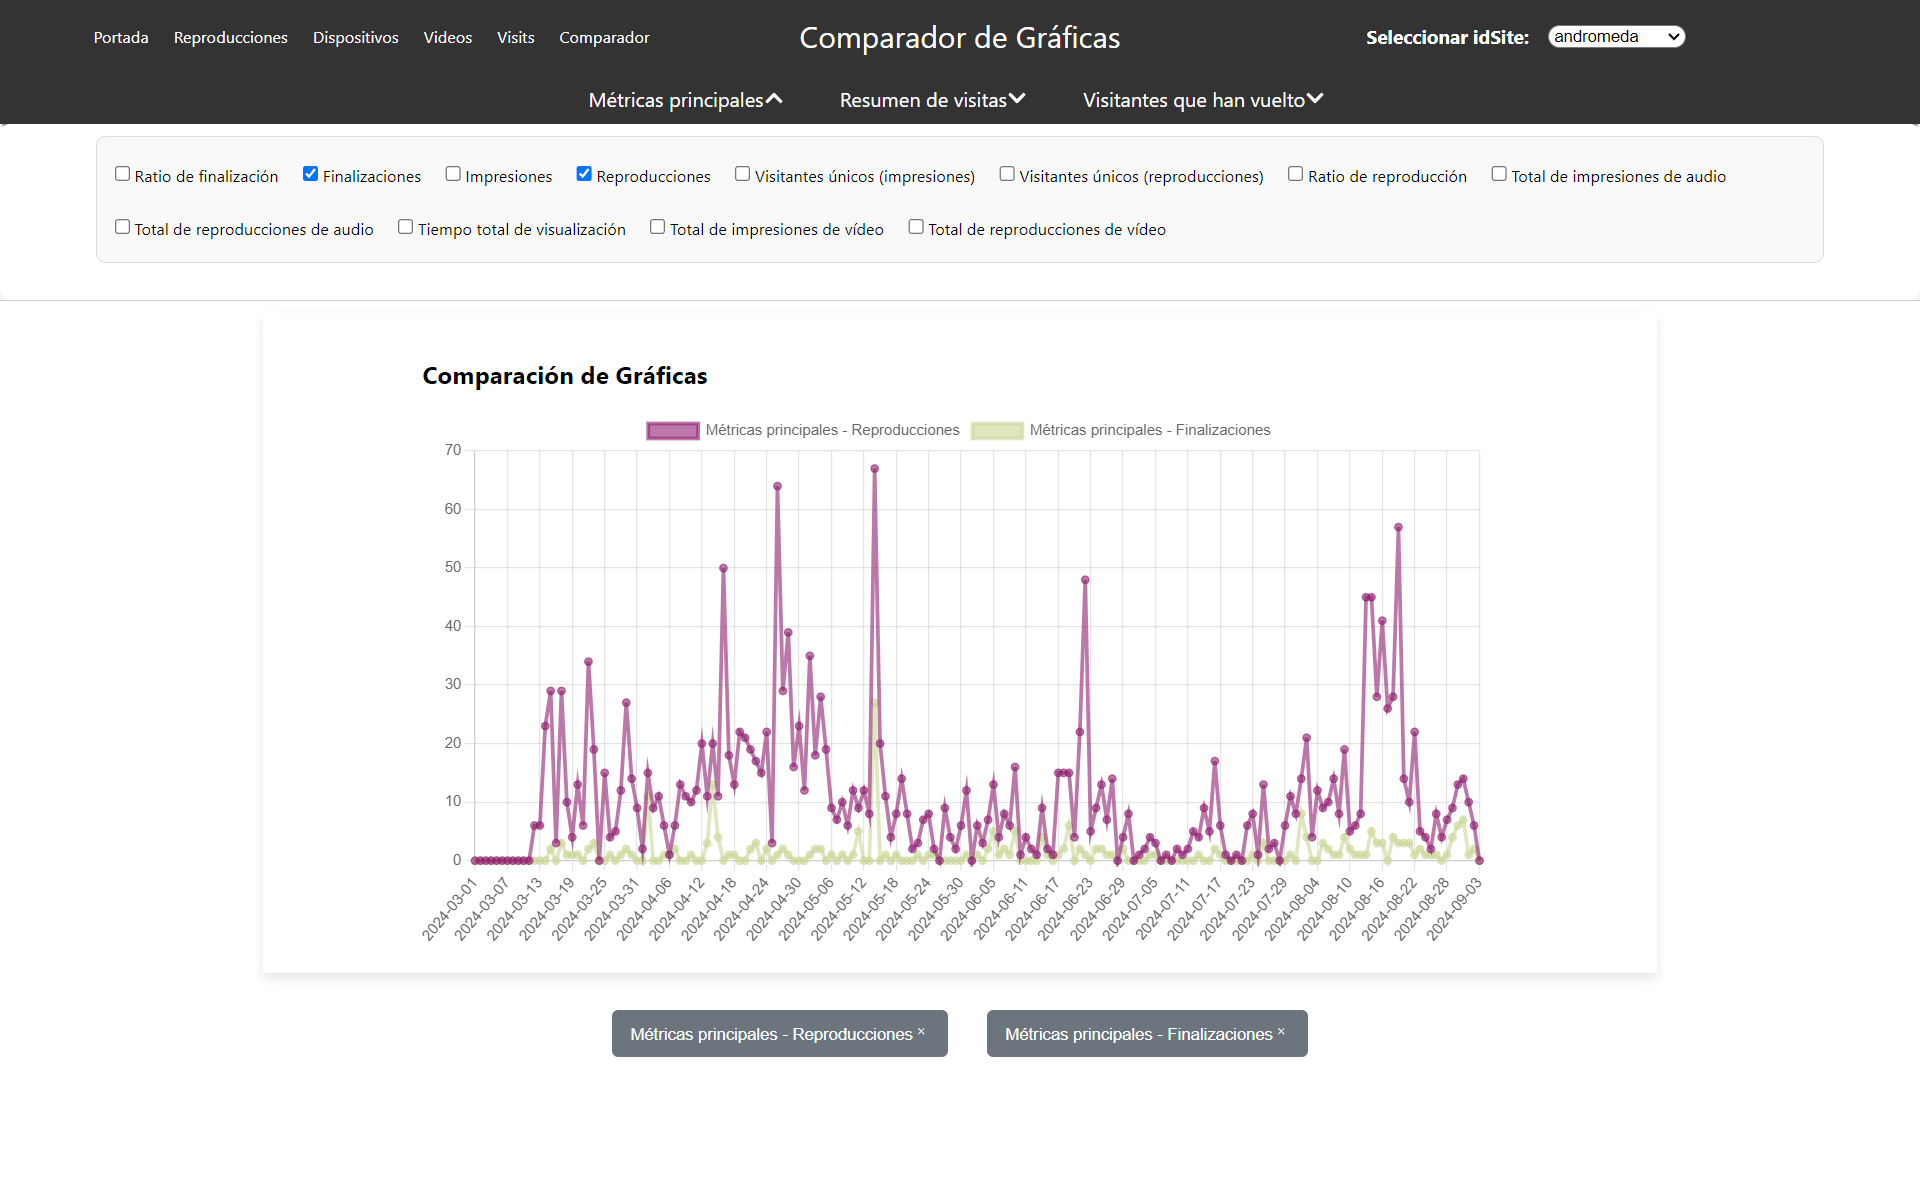
\includegraphics[width=0.8  \textwidth]{imaxes/comparador.png}
    \caption{Página de comparador de la aplicación de análisis de datos}
    \label{fig:comparador}
\end{figure}

El resto de las páginas se dedican a agrupaciones de datos que tienen relación entre sí. La creación de estas páginas se diseñó 
de manera dinámica, permitiendo la creación rápida y sencilla de nuevas secciones. Estas páginas están enfocadas en mostrar 
datos de los visitantes desde diferentes perspectivas. Para una OTT de estas características, pensada para su uso en diversas 
plataformas y dispositivos, una sección relevante es la de dispositivos, que ofrece información sobre los sistemas operativos, 
marcas y modelos desde los cuales se accede. Otro punto clave son las reproducciones, donde se muestra información sobre la 
visualización de contenidos, como el número de reproducciones, tiempo de visualización y los videos más vistos.


\begin{figure}[ht]
    \centering
    \begin{minipage}[b]{0.45\textwidth}
        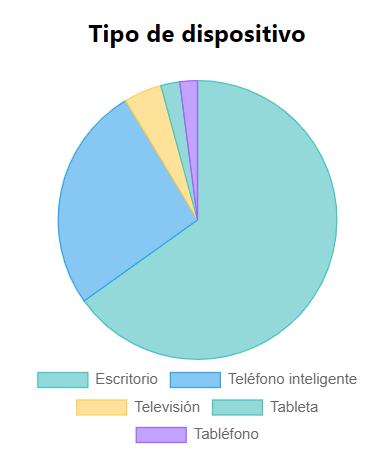
\includegraphics[width=\textwidth]{imaxes/circleGraph.png}
        \caption{Ejemplo de grafico circular mostrando la distribución de los tipos de dispositivos en los que se accede a la web}
        \label{fig:circleGraph}
    \end{minipage}
    \hfill
    \begin{minipage}[b]{0.45\textwidth}
        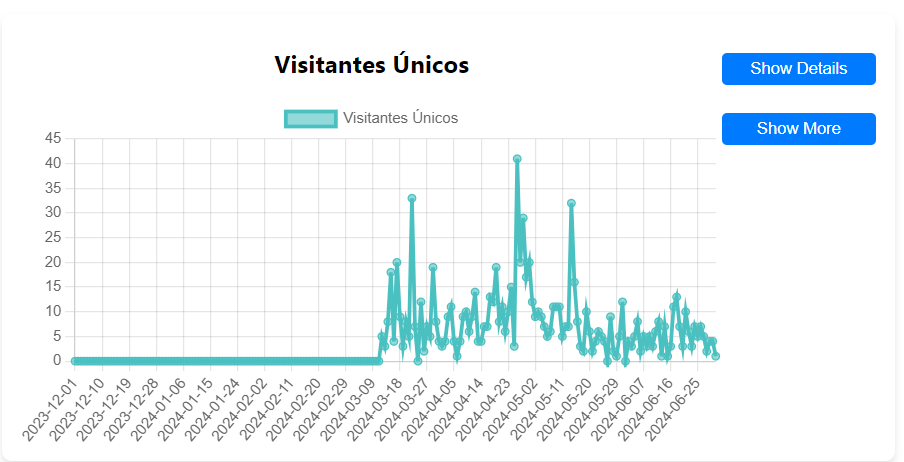
\includegraphics[width=\textwidth]{imaxes/lineGraph.png}
        \caption{Ejemplo de gráfico lineal mostrando la evolución del número de visitantes únicos en la web}
        \label{fig:imagen2}
    \end{minipage}
\end{figure}

Con los enfoques y datos claramente definidos, se procedió al diseño de las páginas y secciones, centrándose en las funcionalidades de la API de 
Matomo que permiten obtener los datos necesarios. Tras analizar las funcionalidades disponibles, y considerando cuáles ya estaban implementadas y 
optimizadas en los sistemas de la empresa, se desarrollaron las pantallas de reproducciones, dispositivos, videos, visitas, además del dashboard 
de inicio y el comparador.

\begin{itemize} 
    \item \textbf{Inicio:} Esta página presenta los gráficos más generales y resumidos de los datos, como el número de visitas, 
    reproducciones y dispositivos en tiempo real. Está diseñada para ofrecer al usuario una visión global de los datos de un solo vistazo. 
    \item \textbf{Reproducciones:} Aquí se muestran gráficos relacionados con las reproducciones de videos, incluyendo el número de reproducciones, 
    tiempo medio de visualización y visitantes únicos. El objetivo es que el usuario pueda analizar los patrones de visualización y obtener insights 
    sobre el comportamiento de los usuarios. 
    \item \textbf{Dispositivos:} En esta página se despliegan gráficos relacionados con los dispositivos desde los que se accede a la web, como 
    sistemas operativos, marcas y modelos. Esto permite al usuario analizar las preferencias de los usuarios en cuanto a dispositivos. 
    \item \textbf{Videos:} Esta página incluye una lista de los contenidos de la plataforma con información detallada de cada uno, como número de 
    reproducciones, tiempo medio de visualización y tasa de finalización. Además, la tabla permite ordenar los datos por diferentes campos, facilitando el análisis. 
    \item \textbf{Visitas:} Esta sección está compuesta por varias páginas que detallan la información sobre las visitas a la web. Actualmente incluye 
    páginas dedicadas a resumen de visitas, tiempo de navegación, frecuencia de visitas e interés de los visitantes. 
    \item \textbf{Comparador:} En esta página el usuario puede visualizar y comparar gráficos de diferentes módulos para analizar correlaciones, 
    tendencias o patrones entre los datos. Esto facilita la obtención de insights sobre la relación entre diferentes variables y módulos, ayudando 
    a tomar decisiones informadas. 
\end{itemize}


\subsubsection{Funcionalidades de la aplicación}
\label{sec:diseno-funcionalidades}

Además de la visualización de gráficos y tablas, la aplicación incluye una funcionalidad que permite al usuario obtener explicaciones sobre los 
datos que se están mostrando. Esta opción ofrece tanto una breve descripción como un análisis más detallado de los datos a través de la API de OpenAI.

Para generar este análisis, se utiliza un contexto general de la sección de la aplicación desde la cual se visualizan los datos, complementado con 
la información de la gráfica específica. Este contexto, que incluye metadatos relacionados con los usuarios y las interacciones dentro de la OTT, se 
almacena en MongoDB. Así, a medida que se va utilizando la plataforma, este contexto se enriquece y se optimiza para proporcionar análisis cada vez más 
precisos y detallados



